\documentclass[12pt]{article}


% Math		****************************************************************************************
\usepackage{fancyhdr} 
\usepackage{amsfonts}
\usepackage{amsmath}
\usepackage{amsthm}
\usepackage{dsfont}

% Macros	****************************************************************************************
\usepackage{calc}

% Commands	****************************************************************************************
%\newcommand{\problem}[1]{\hspace{-\widthof{#1}} \textbf{#1}}
\newcommand{\problem}[1]{\hspace{-4 ex} \large \textbf{#1}\\}
\newcommand{\reverseconcat}[3]{#3#2#1}

%page		****************************************************************************************
\usepackage[margin=1in]{geometry}
\usepackage{setspace}
\doublespacing
\pagestyle{fancy}
\fancyhf{}
\rhead{Shaw \space \thepage}
\setlength\parindent{0pt}

%Code		****************************************************************************************
\usepackage{listings}
\usepackage{courier}
\lstset{
	language=Python,
	showstringspaces=false,
	formfeed=newpage,
	tabsize=4,
	commentstyle=\itshape,
	basicstyle=\ttfamily,
}

%Images		****************************************************************************************
\usepackage{graphicx}
\graphicspath{ {images/} }


\begin{document}
	\thispagestyle{empty}
	
	\begin{flushright}
		Sage Shaw \\
		m565 - Fall 2017 \\
		\today
	\end{flushright}
	
{\large \textbf{HW 2}}\bigbreak

\problem{1 (a)}\\
	Code for secant method in python follows:
	\singlespacing
	\begin{lstlisting}
def secant(f, x0, x1, epsilon=1e-16, n_max=10**5):
	xs = [x0,x1]
	xn = x1
	xn_1 = x0
	fn = f(xn)
	fn_1 = f(xn_1)
	for i in range(n_max):
		if abs(fn) < epsilon:
			return xs[-1], len(xs)
		xn, xn_1 = xn - (xn-xn_1)/(fn-fn_1)*fn, xn
		fn, fn_1 = f(xn), f(xn_1)
		xs.append(xn)
	return None
	\end{lstlisting}
	\doublespacing
	
\problem{1 (b)}
	Code for Newton's method in python follows:
	\singlespacing
	\begin{lstlisting}
def newton(f, df, x0, epsilon=1e-16, n_max=10**5):
	x = x0
	xs =[x]
	fx = f(x)
	dfx = df(x)
	for i in range(n_max):
		if abs(fx) < epsilon:
			return xs[-1], len(xs)
		x = x - fx/dfx
		xs.append(x)
		fx, dfx = f(x), df(x)
	return None
	\end{lstlisting}
	\doublespacing
\problem{1 (c)}\\
	The output for the secant method is below.
	\begin{center}
		\begin{tabular}{|c|c|c|c|}
			\hline
			$n$&$x_n$&relative error&rate\\ \hline
			1&5.5&8.6977255889355&N/A\\ \hline
			2&5.25&8.256919880347523&N/A\\ \hline
			3&0.0294863000416&0.948009082466&-0.0252912792622\\ \hline
			4&0.823978157018&0.452857101461&14.8372523985\\ \hline
			5&0.593254095941&0.0460391685359&3.88581886785\\ \hline
			6&0.565982615568&0.00204652838394&2.01139762445\\ \hline
			7&0.567148753391&9.63245318171e-06&1.86548763383\\ \hline
			8&0.567143291557&2.02338959262e-09&1.73314683194\\ \hline
			9&0.56714329041&4.89392647061e-15&1.64601718863\\ \hline
		\end{tabular}
	\end{center}
	It's somewhat difficult to tell with so few iterations, but the rate of convergence appears to be approaching the golden ratio as expected.

	The output for Newton's method is below.
	\begin{center}
	    \begin{tabular}{|c|c|c|c|}
	    	\hline
	    	$n$&$x_n$&relative error&rate\\ \hline
	    	1&5.25&8.256919880347523&N/A\\ \hline
	    	2&0.0326257855847&0.942473469868&-0.0280654002561\\ \hline
	    	3&0.507891082956&0.104474845169&38.1249608767\\ \hline
	    	4&0.566496637787&0.00114019267083&3.00005806752\\ \hline
	    	5&0.56714321473&1.33440892109e-07&2.33593620286\\ \hline
	    	6&0.56714329041&5.08968352943e-15&2.07911417502\\ \hline
	    \end{tabular}
	\end{center}
    It's somewhat difficult to tell with so few iterations, but it appears to be converging quadratically as expected.
    
\problem{2 (a)}
	Assume that $f$ has a root at $x^*$. Define $\epsilon_n = x^*-x_n$ for each $x_n$. Then $0 = f(x^*) = f(x_n + \epsilon_n)$. By Taylor series expanding around $x_n$ we get that 
	$$
	0 = f(x_n + \epsilon_n) \approx f(x_n) + \epsilon_n f^\prime(x_n) + \frac{\epsilon_n^2}{2}f^{\prime\prime}(x_n)
	$$
	or equivalently
	\begin{align}\label{p2a1}
	\epsilon_n \approx -\frac{f(x_n)}{f^\prime(x_n)} - \frac{\epsilon_n^2f^{\prime\prime}(x_n)}{2f^\prime(x_n)}
	\end{align}
	If we then assume that $\epsilon_n^2 \approx 0$, we can say that $\epsilon_n \approx \frac{-f(x_n)}{f^\prime(x_n)}$. Substituting into the right side of (\ref{p2a1}) we get 
	$$
	x^* - x_n = \epsilon_n \approx -\frac{f(x_n)}{f^\prime(x_n)} - \frac{f(x_n)^2f^{\prime\prime}(x_n)}{2f^\prime(x_n)^3}
	$$
	which gives us the recurrance relation
	$$
	x_{n+1} = x_n -\frac{f(x_n)}{f^\prime(x_n)} - \frac{f(x_n)^2f^{\prime\prime}(x_n)}{2f^\prime(x_n)^3}
	$$
	
\problem{2 (b)}
	Below can be seen the output of a session of Maple. The first two lines verify that Newton's method is quadratically convergent since the error term is $\mathcal{O}(x^3)$. The next two lines verify that our modified Newton's method is cubically convergent since the error term is $\mathcal{O}(x^4)$.
	
	\begin{figure}[h]
		\caption{Maple output}
		\centering
		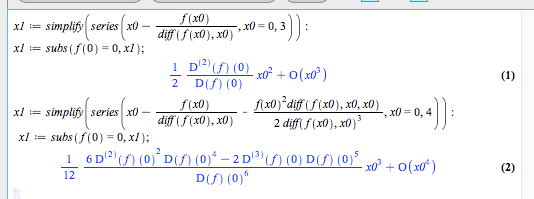
\includegraphics[width=.75\textwidth]{hw2_p3b}
	\end{figure}
	
\problem{3 (a)}
	If $r=1-\frac{x^2}{a}$ then $\sqrt{a} = x(1-r)^{-\frac{1}{2}}$. \\
	Then the iteration $x_{n+1} = x_n(1-r)^{-\frac{1}{2}}$ where $r=1-\frac{x_n^2}{a}$ will converge in one step. If we Taylor expand $f(r) = (1-r)^{-\frac{1}{2}}$ around $r=0$ we get
	$$
	f(r) = (1-r)^{-\frac{1}{2}} \approx 1 + \frac{1}{2}r
	$$
	Substituting back $r=1-\frac{x_n^2}{a}$ we get $f(1-\frac{x_n^2}{a}) \approx 1 + \frac{1}{2} (1-\frac{x_n^2}{a}) = \frac{1}{2}(3-\frac{x_n^2}{a})$. Then our iteration becomes $x_{n+1} = \frac{x_n}{2}(3-\frac{x_n^2}{a})$. This is iterating on the function $y=\frac{3}{2}x - \frac{1}{2a}x^3$. Note that the derivative is $y^\prime = \frac{3}{2} - \frac{3}{2a}x^2$ and it is easy to see that $y^\prime(\sqrt{a}) = 0$. Since the derivative is zero at our roo, we will get quadratic convergence. My Python implementation follows.
	\singlespacing
	\begin{lstlisting}
def my_sqrt(a, x0, epsilon=1e-15, n_max=10**5):
	xs = [x0]
	x = x0
	for i in range(n_max):
		if abs(x**2 - a) < epsilon:
			return xs
		x = x/2 * (3 - x**2/a)
		xs.append(x)
	return  None
	\end{lstlisting}\doublespacing
	
	The output can be seen below for $a=2$ and $x_0=1$. After a few iterations the number of accurate digits almost doubles at each iteration, consistent with quadratic convergence.
	
	\begin{center}
		\begin{tabular}{|c|c|c|c|}
			\hline
			$n$&$x_n$&abs err&ratio\\ \hline
			1&1&0.414213562373&N/A\\ \hline
			2&1.25&0.164213562373&2.04974089911\\ \hline
			3&1.38671875&0.0274948123731&1.98925208746\\ \hline
			4&1.413416936993599&0.000796625379496&1.98542199024\\ \hline
			5&1.4142128893918142&6.72981280925e-07&1.99177257226\\ \hline
			6&1.4142135623726146&4.80504525058e-13&1.99583740676\\ \hline
			7&1.4142135623730951&0.0&N/A\\ \hline
		\end{tabular}
	\end{center}
	
\problem{3 (b)}
	In Figure 1 can be seen equation (3) from the homework: $y=\frac{1}{2}(x+\frac{a}{x})$.
	\begin{figure}[h]
		\caption{$y=\frac{1}{2}(x+\frac{a}{x})$ and $y=x$}
		\centering
		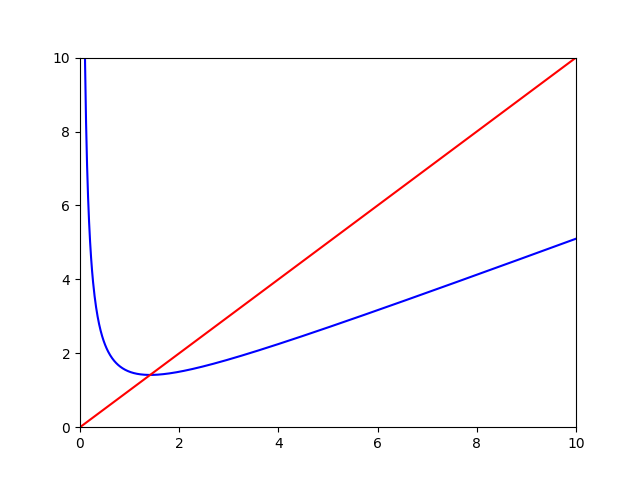
\includegraphics[width=.5\textwidth]{hw2_figure_1}
	\end{figure}\\
	Note, that for a square-root, only a positive valued initial guess is appropriate. From the graph, one would expect that all choices of starting point will converge. The table below confirms this suspicion. 
	\begin{center}
		\begin{tabular}{|c|c|}
			\hline
			$x_0$&converged\\ \hline
			0.0001&1.414213562373095\\ \hline
			1&1.414213562373095\\ \hline
			2&1.414213562373095\\ \hline
			4&1.414213562373095\\ \hline
			100&1.414213562373095\\ \hline
		\end{tabular}
	\end{center}
	
	In Figure 2 can be seen equation (4): $y=\frac{x}{2}(3-\frac{x^2}{a})$.
	\begin{figure}[h]
		\caption{$y=\frac{x}{2}(3-\frac{x^2}{a})$ and $y=x$}
		\centering
		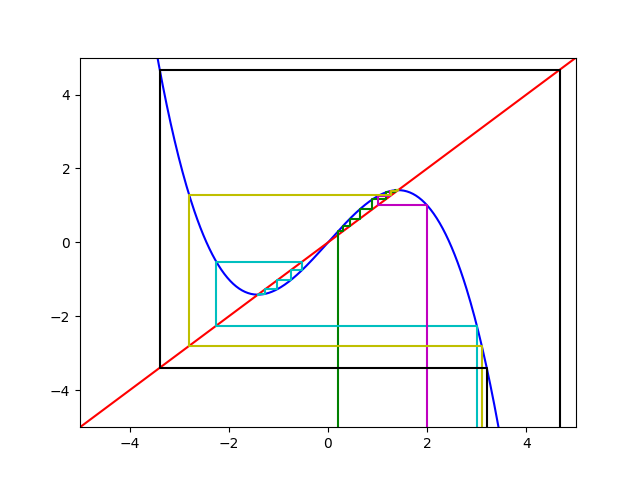
\includegraphics[width=.75\textwidth]{hw2_figure_2}
	\end{figure}
	From the figure it is clear that a choice of $x_0 \in (0,\sqrt{2})$ will converge to $\sqrt{2}$. Also, after that interval there is a short interval where the first iteration gets mapped into $(0,\sqrt{2})$ The function has a root at $\sqrt{6}$ so $x_0 \in (0,\sqrt{6})$ will converge to $\sqrt{2}$. This can be seen numerically in the table below.
	
	\singlespacing
	\begin{center}
		\begin{tabular}{|c|c|}
			\hline
			$x_0$&converged\\ \hline
			0&0.0\\ \hline
			0.01&1.4142135623730951\\ \hline
			1&1.414213562373095\\ \hline
			1.41421356237&1.41421356237\\ \hline
			2&1.414213562373095\\ \hline
			2.44848974278 $<\sqrt{6}$&1.41421356237\\ \hline
			2.45048974278$>\sqrt{6}$&-1.41421356237\\ \hline
		\end{tabular}
	\end{center}
	\doublespacing
	
	From the graph we can see that there are some choices of starting values greater than $\sqrt{6}$ whose second iteration maps it to the interval $(0,\sqrt{6})$ and will thus converge. There will be an infinite sequence of increacingly small intervals somewhere inside of $(\sqrt{6}, 3)$ whose second iteration will land in the previous interval and will thus converge to $\sqrt{2}$ by induction. 
	
	
\problem{3 (c)}
	Notice that similarly to above, $\frac{1}{\sqrt{a}}=x(1-r)^{-\frac{1}{2}}$ where $r=1-ax^2$ is an identity for any positive value of $x$. We then Taylor expand the function $f(r)=(1-r)^{-\frac{1}{2}}$ about $r=0$ to get the following
	$$
	f(r) \approx 1 + \frac{1}{2}r + \frac{3}{8}r^2
	$$
	Substituting $r=1-ax^2$ we get
	\begin{align*}
		f(1-ax^2) & \approx 1 + \frac{1}{2}(1-ax^2) + \frac{3}{8}(1-ax^2)^2\\
		& \approx 1 + \frac{1}{2} - \frac{a}{2}x^2 + \frac{3}{8}(1-2ax^2 + a^2x^4) \\
		& \approx 1 + \frac{1}{2} - \frac{a}{2}x^2 + \frac{3}{8} -\frac{6}{8}ax^2 + \frac{3}{8}a^2x^4) \\
		& \approx \frac{15}{8} - \frac{10}{8}ax^2 + \frac{3}{8}a^2x^4\\
		& \approx \frac{1}{8}(15 - 10ax^2 + 3a^2x^4)\\
		& \approx \frac{1}{8}(15 - ax^2(10 - 3ax^2))
	\end{align*}
	Then our iteration becomes
	\begin{align*}
		x_{n+1} & = x_nf(1-ax_n^2) \\
		x_{n+1} & = \frac{x_n}{8}(15 - ax_n^2(10 - 3ax_n^2))
	\end{align*}
	as desired. The implied function is $y=\frac{1}{8}(15x - 10ax^3 + 3a^2x^5)$. Note its derivatives $y^\prime = \frac{1}{8}(15 - 30ax^2 + 15a^2x^4)$ and $y^{\prime\prime} = \frac{1}{8}(-60ax + 60a^2x^3)$. We can see that
	
	\begin{align*}
		y^\prime \Bigg(\frac{1}{\sqrt{a}} \Bigg) & = \frac{1}{8} \Bigg[15 - 30a \Bigg(\frac{1}{\sqrt{a}} \Bigg)^2 + 15a^2 \Bigg(\frac{1}{\sqrt{a}} \Bigg)^4 \Bigg] \\
		& = \frac{1}{8}(15 - 30 + 15) \\
		& = 0
	\end{align*}
	and 
	\begin{align*}
	y^{\prime\prime} \Bigg(\frac{1}{\sqrt{a}} \Bigg) & = \frac{1}{8}\Bigg[-60a \Bigg(\frac{1}{\sqrt{a}} \Bigg)+ 60a^2 \Bigg(\frac{1}{\sqrt{a}} \Bigg)^3\Bigg] \\
	& = y^{\prime\prime} = \frac{1}{8}(-60\sqrt{a} + 60\sqrt{a}) \\
	& = 0
	\end{align*}
	Since the first and second derivatives are 0 at our fixed point, we can expect cubic convergence.
	
	
	
\problem{4}
	Suppose $f(x)$ has a root of multiplicity $p>1$ at $x^*$. Then by definition there exists a function $g(x)$ such that $f(x) = (x-x^*)^pg(x)$ and $g(x^*) \neq 0$. Then $f^\prime(x) = (x-x^*)^pg^\prime(x) + p(x-x^*)^{p-1}g(x)$. Now let 
	\begin{align*}
		\mu(x) & = \frac{f(x)}{f^\prime(x)} \\
		& = \frac{(x-x^*)^pg(x)}{(x-x^*)^pg^\prime(x) + p(x-x^*)^{p-1}g(x)} \\
		& = \frac{(x-x^*)g(x)}{(x-x^*)g^\prime(x) + pg(x)}
	\end{align*}
	
	Then $\mu(x)$ is only equal to zero when the numerator $(x-x^*)g(x)$ is equal to zero. Since $g(x)$ does not have a root at $x^*$, by definition $\mu(x)$ has a root of multiplicity 1 at $x^*$. Thus Newton's method on $\mu(x)$ will converge to $x^*$ quadratically. 
	
\problem{5 (a)}
	From the table below it can be seen that that the iteration occilates between 0.9948 and 0.0117. Obviously neither of these are a solution to our problem since the next iteration returns the other number for each. 
	\singlespacing
	\begin{center}
		\begin{tabular}{|c|c|}
			\hline
			$n$&$x_n$\\ \hline
			1&0\\ \hline
			2&0.9953222650189527\\ \hline
			3&0.010556209425946548\\ \hline
			4&0.9948670503002457\\ \hline
			\vdots & \vdots \\ \hline
			26&0.9948153975507391\\ \hline
			27&0.011699975456613668\\ \hline
			28&0.9948153975507384\\ \hline
			29&0.011699975456615172\\ \hline
			30&0.9948153975507384\\ \hline
		\end{tabular}
	\end{center}
	\doublespacing
	
	\clearpage
	
\problem{5 (b)}
	Python implementation of Steffenson's iterative method:
	\singlespacing
	\begin{lstlisting}
def foo_6(x):
	return -1*erf(2*(x-1))
	
def hw2_p5b():
	xs = [0]
	x = 0
	ns = [0]
	#perform first iteration so that 
#error checking can compute
	g = foo_6(x)
	x = x - (g-x)**2/(foo_6(g) -2*g + x)
	xs.append(x)
	for i in range(1,1000000): 
		if abs(xs[-1] - xs[-2]) < 1e-15:
			break
		g = foo_6(x)
		if abs((foo_6(g) -2*g + x)) < 1e-15:
			break
		x = x - (g-x)**2/(foo_6(g) -2*g + x)
		xs.append(x)
		ns.append(i)
	latex_table((ns, xs),('$n$', '$x_n$'))
	\end{lstlisting}
	\doublespacing
	Iterations of Steffenson's iterative method are in the the table below.
	\begin{center}
		\begin{tabular}{|c|c|}
			\hline
			$n$&$x_n$\\ \hline
			0&0\\ \hline
			1&0.5003142541320008\\ \hline
			2&0.6395901752177244\\ \hline
			3&0.661032522348998\\ \hline
			4&0.6615598346647998\\ \hline
			5&0.6615601506706955\\ \hline
			6&0.661560150670809\\ \hline
		\end{tabular}
	\end{center}

\problem{5 (c)}
	From the fundamental theorem of calculus 
	$$
	\frac{d}{dx}\text{erf}(x) = \frac{d}{dx}\frac{2}{\sqrt{\pi}}\int_0^x e^{-t^2}dt = \frac{2}{\sqrt{\pi}} e^{-x^2}
	$$
	Using this and applying the chain rule, we arive at the derivative of $g(x) = -\text{erf}(2(x-1))$ \\
	$$
	g^\prime(x) = -\frac{4}{\sqrt{\pi}} e^{-x^2}
	$$
	Evaluating at our fixed point $x^* = 0.661560150670809$ we obtain $g(x^*) = -1.4272696617560152$. Since the magnitude of this derivative is not less than 1, we are not guaranteed convergence by the Fixed Point theorem. 	
	
\problem{6} 
	Suppose we have a function $f(x)$, such that for any $x_0$, an iteration of Newton's method returns $-x_0$. That is 
	$$
	-x_0 = x_0 - \frac{f(x)}{f^\prime(x)}
	$$
	It then follows that $2x_0 = \frac{f(x)}{f^\prime(x)}$. Letting $f(x)=y$, we can then manipulate it as follows
	\begin{align*}
		\frac{1}{y}\frac{dy}{dx} & = \frac{1}{2x} \\
		\int \frac{1}{y}\frac{dy}{dx} dx & = \int \frac{1}{2x} dx \\
		\int \frac{1}{y}dy & = \frac{1}{2}\int \frac{1}{x} dx \\
		ln\vert y \vert & = \frac{1}{2} ln\vert x \vert + C_0 \\
		ln\vert y \vert & = ln\vert x \vert^\frac{1}{2} + C_0 \\
		\vert y \vert & = C_1 \vert x \vert^\frac{1}{2} \\
		y & = \pm C_1 \sqrt{\vert x \vert} \\
	\end{align*}
	Noticing that the derivative is undefined at $x=0$ we allow for separate solutions when $x$ is either positive or negative. One can quickly check that the choice $f(x)=C_1 \text{sign}(x)\sqrt{\vert x \vert}$ is the desired general solution.

\problem{7 (a)}
	Consider the fixed point iteration $x_{n+1}=e^{x_n}-1$. This is attempting to find a fixed point for the function $y=e^x-1$. From our Fixed Point Theorem we are only guaranteed convergence when the magnitude of the derivative is less than 1 on the entire interval. Since $y^\prime=e^x$ we know that $y^\prime<1$ on the interval $(-\infty,0)$. Also $y((-\infty,0]) = (-1,0] \subseteq (-\infty,0]$. Thus all of our iterations will be in $(-\infty,0]$. Using the Fixed Point Theorem is difficult however since there is no maximum of $\vert y^\prime \vert $ on the open interval $(-\infty,1)$ and the supremum is equal to 1. \bigbreak
	
	We will take another approach. \bigbreak
	
	For $x_n\leq-1$, we know that $x_n\leq-1< e^{x_n}-1 = x_{n+1}$. We would like to show that $x_n<e^{x_n}-1$ when $-1 < x_n < 0$ as well. Consider the Taylor Series expansion of $e^{x_n}-1 = x_n + \sum\limits_{i=2}^\infty \frac{x_n^i}{n!}$. The even powered terms of this series will be positive and the odd will be negative. Since the magnitude of each term is greater than the term it precedes, and it starts on an even term, the sum will be positive. Thus $x_n<e^{x_n}-1=x_{n+1}$. Since this series is monotonically increasing and it is bounded above it converges. \bigbreak
	
	Hence, our iterations will converge for $x_0 \in (-\infty,0)$.
	
\problem{7 (b)}
	From the Taylor Expansion of $e^x$ we know that 
	$$e^{x_n} =  1 + x_n + x_n^2/2 + \mathcal{O}(x_n^3)$$
	and $x_{n+1} = e^{x_n}-1 \approx x_n + x_n^2/2$. Then $\frac{x_{n+1} - x_n}{1} \approx x_n^2/2$. This can be thought of as a secant line to a continuous function $x(t)$ where $x(n) = x_n$ for large $n$. Since all $x_n$ are approaching $0$, this secant line is becoming a close approximation of the derivative. Consider the differential equation $\frac{dx}{dt} = \frac{1}{2}x^2$. This equation is separable and solvable as follows
	\begin{align*}
		x^{-2}\frac{dx}{dt} & = \frac{1}{2} \\
		\int x^{-2}\frac{dx}{dt} dt & = \int \frac{1}{2} dt \\
		\int x^{-2}dx & = \int \frac{1}{2} dt \\
		-x^{-1} & = \frac{1}{2}t - C \\
		x & = \frac{1}{C - \frac{1}{2}t} \\
	\end{align*}
	Using the known evaluation $x(0)=x_0$ we get $x_0=1/C$ which gives us a general solution
	$$
	x = \frac{1}{\frac{1}{x_0} - \frac{1}{2}t}
	$$
	One can argue that for large $n$ this approximation gives us 
	$$x_n = \frac{1}{\frac{1}{x_0} - \frac{1}{2}n}$$
	We would like to know a value of $n$ sufficient to make $\vert x_n-0\vert < \epsilon$ for a small positive $\epsilon$. Since $x_n<0$ we need $x_n>-\epsilon$. Then
	\begin{align*}
		-\epsilon &< \frac{1}{1/x_0 - 1/2n} \\
		1 & > \frac{-1}{\epsilon} \frac{1}{1/x_0 - 1/2n} \\
		\frac{1}{x_0} - \frac{1}{2}n & < \frac{-1}{\epsilon}\\
		- \frac{1}{2}n & < -\frac{1}{\epsilon} - \frac{1}{x_0}\\
		n & > \frac{2}{\epsilon} + \frac{2}{x_0}
	\end{align*}
	Close choices of $x_0$ can reduce the required itterations since $\frac{2}{x_0}$ is negative, but for most choices  $\frac{2}{\epsilon}$ dominates. To get within $10^{-10}$ of the root, we would expect something around $2 \times 10^{10}$ (20 billion) iterations. Since it is somewhat impractical to check this calculation we will instead attempt to verify our formula for predicting the number of iterations by using larger $\epsilon$s and better $x_0$s. The results are recorded in the table below.
	
	\begin{center}
		\begin{tabular}{|c|c|c|c|c|}
			\hline
			$\epsilon$&$x_0$&$n$ predicted&$n$ actual&relative error\\ \hline
			0.0001&-0.1&20020&19978&0.21\%\\ \hline
			1e-05&-0.1&200020&199977&0.02\%\\ \hline
			1e-06&-0.1&2000020&1999977&0.00\%\\ \hline
			0.0001&-0.01&20200&19799&2.03\%\\ \hline
			1e-05&-0.01&200200&199798&0.20\%\\ \hline
			1e-06&-0.01&2000200&1999797&0.02\%\\ \hline
			0.0001&-0.001&22000&18000&22.22\%\\ \hline
			1e-05&-0.001&202000&197999&2.02\%\\ \hline
			1e-06&-0.001&2002000&1997998&0.20\%\\ \hline
		\end{tabular}
	\end{center}
	
	It looks like the error in our prediction begins to become significant when $x_0$ gets sufficiently close to $0$. Otherwise our predictions are becoming more accurate as $\epsilon$ becomes smaller. Based on these results we can expect that our prediction of roughly 20 billion iterations will be close to but slightly higher than the actual number of iterations for reasonable choices of $x_0$.
	
	
	
	

\end{document}
